\documentclass{article}

\usepackage{amsfonts}
\usepackage{amsmath}
\usepackage{hyperref}
\usepackage{mathtools}
\usepackage{tikz}

\usetikzlibrary{arrows}
\usetikzlibrary{positioning}
\usetikzlibrary{trees}

\title{R1CS Programming \\ \large ZK0x04 Workshop Notes}
\author{Daniel Lubarov \and Brendan Farmer}
\date{\today}

\DeclarePairedDelimiter\ceil{\lceil}{\rceil}
\DeclarePairedDelimiter\floor{\lfloor}{\rfloor}

% Hyperlink colors.
\hypersetup{
    colorlinks=true,
    linkcolor=blue,
    citecolor=blue,
    urlcolor=blue,
}

% Tweak autoref names to use capitals.
\renewcommand{\sectionautorefname}{Section}

\begin{document}

\maketitle

{\hypersetup{hidelinks} \tableofcontents}
\newpage


\section{Multiplicative inverse} \label{sec:inverse}

Deterministically computing $1 / x$ in an R1CS circuit would be expensive. Instead, we can have the prover compute $1 / x$ outside of the circuit and supply the result as a witness element, which we will call $x_\mathrm{inv}$. To verify the result, we enforce
\begin{equation}
  (x) (x_\mathrm{inv}) = (1)
\end{equation}


\section{Zero testing} \label{sec:zerotest}

To assert $x = 0$, we simply enforce
\begin{equation}
  (x) (1) = (0)
\end{equation}
Asserting $x \ne 0$ is similarly easy: we compute $1 / x$ (non-deterministically, as in \autoref{sec:inverse}). The result can be ignored; the mere fact that an inverse exists implies $x \ne 0$.

On the other hand, if we want to \textit{evaluate}
\begin{equation} \label{eq:nonzero}
  y \coloneqq
  \begin{cases}
    0 & \text{if $x = 0$,} \\
    1 & \text{otherwise,}
  \end{cases}
\end{equation}
we can do so by introducing another variable, $m$, and enforcing
\begin{alignat}{2}
  (x)     & (m) &&= (y), \\
  (1 - y) & (x) &&= (0).
\end{alignat}
Outside of the circuit, the prover generates $y$ as in \autoref{eq:nonzero}, and generates $m$ as
\begin{equation}
  m \coloneqq
  \begin{cases}
    1 & \text{if $x = 0$,} \\
    y / x & \text{otherwise.}
  \end{cases}
\end{equation}
This method is from \cite{parno2013pinocchio}.

We can also use this technique to test for equality, since $x = y$ if and only if $x - y = 0$.


\section{Binary}

To assert $b \in \{ 0, 1 \}$, we enforce
\begin{equation} \label{eq:boolean}
  (b) (b - 1) = (0).
\end{equation}

To ``split'' a field element $x$ into its binary encoding, $(b_1, \dots, b_n)$, we have the prover generate the binary encoding out-of-band. We then verify it by applying \autoref{eq:boolean} to each $b_i$, and enforcing
\begin{equation} \label{eq:binary}
  (x) (1) = \left( \sum_{i=0}^{n-1} 2^i b_i \right),
\end{equation}
assuming a little-ending ordering of the bits.

Note that \autoref{eq:binary} permits two encodings of certain field elements. In $\mathbb{F}_{13}$ for example, the element $1$ can be represented as either $0001$ or $1110$. If a canonical encoding is required, we can prevent ``overflowing'' encodings by asserting that $(b_1, \dots, b_n) < |F|$. Such binary comparisons are covered in \autoref{sec:comparisons}.

To ``join'' a sequence of bits into the field element they encode, we simply take a weighted sum of the bits:
\begin{equation} \label{eq:join}
  x \coloneqq \sum_{i=0}^{n-1} 2^i b_i.
\end{equation}
This does not require any constraints, unless we don't know whether $(b_1, \dots, b_n)$ is the canonical encoding of some field element, in which case we may want a comparison to assert that overflow does not occur.


\section{Selection} \label{sec:selection}

Suppose we have a boolean value $s$, and we wish to compute
\begin{equation}
  z \coloneqq
  \begin{cases}
    x & \text{if $s = 0$,} \\
    y & \text{if $s = 1$.}
  \end{cases}
\end{equation}
We can compute this as
\begin{equation} \label{eq:selection}
  z \coloneqq x + s(y - x).
\end{equation}
This requires two constraints: one ``is boolean'' asertion (\autoref{eq:boolean}), assuming $s$ was not already known to be boolean, and another for the multiplication.


\section{Random access}

Suppose we have a sequence $S = (x_0, \dots, x_n)$, and we wish to access the $i$th element. One approach would be to multiply each element by an equality test (\autoref{sec:zerotest}) comparing that element's index to $i$, then sum up those products. In particualar,
\begin{equation}
  S_i = \sum_{j=0}^{n-1} (i = j) x_j
\end{equation}
This requires $3n$ constraints: $2n$ for the zero tests and $n$ for the products.

A better approach is to split $i$ into its binary encoding, $(i_0, \dots, i_k)$, where $k = \ceil{\log_2 n}$. Then we can view $(i_0, \dots, i_k)$ as a path through a binary tree with $(x_0, \dots, x_n)$ as its leaves. For example, if $n = 4$, we could imagine the following binary tree:
\begin{center}
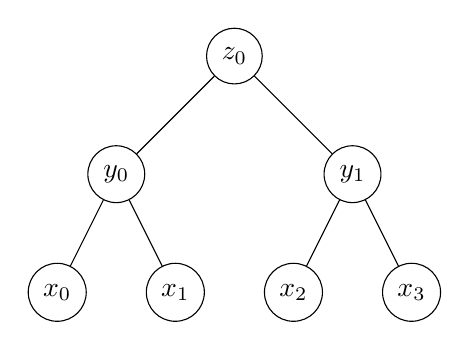
\begin{tikzpicture}[level distance=1.5cm,
  level 1/.style={sibling distance=3cm},
  level 2/.style={sibling distance=1.5cm}]
  \node[circle,draw] {$z_0$}
    child {node[circle,draw] {$y_0$}
      child {node[circle,draw] {$x_0$}}
      child {node[circle,draw] {$x_1$}}
    }
    child {node[circle,draw] {$y_1$}
      child {node[circle,draw] {$x_2$}}
      child {node[circle,draw] {$x_3$}}
    };
\end{tikzpicture}
\end{center}
Then for each non-leaf node, we would select one of its two children using the method from \autoref{sec:selection}. In the example, we have
\begin{alignat}{2}
  y_0 &\coloneqq x_0 + b_0 (x_1 - x_0), \\
  y_1 &\coloneqq x_2 + b_0 (x_3 - x_2), \\
  z_0 &\coloneqq y_0 + b_1 (y_1 - y_0).
\end{alignat}

If $n$ is a power of 2, this method takes $\log_2 n + 1$ constraints for splitting $i$ and $n - 1$ constraints for the selection operations, for a total cost of $n + \log_2 n$. If $(x_0, \dots, x_n)$ is comprised of constant values, then selecting between two leaf nodes becomes a free linear combination, saving us $n / 2$ constraints.

If $n$ is not a power of 2, this method can still be used, but we need to think about how to handle out-of-bounds indices. We could assert $i \le n$ (\autoref{sec:comparisons}), but this may not be necessary depending on the context.


\section{2x2 switch}

Suppose we wish to implement a switch with the following structure:
\begin{center}
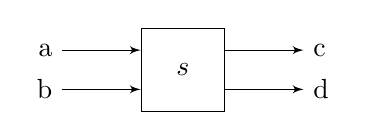
\begin{tikzpicture}[node distance=1.0cm,auto,>=latex']
  \node [draw, minimum size=3em] (s) {$s$};
  \node (a) [left=of s.155] {a};
  \node (b) [left=of s.205] {b};
  \node (c) [right=of s.25] {c};
  \node (d) [right=of s.335] {d};
  \draw[->] (a) -- (s.155);
  \draw[->] (b) -- (s.205);
  \draw[->] (s.25) -- (c);
  \draw[->] (s.335) -- (d);
\end{tikzpicture}
\end{center}
In particular, if $s = 0$ then the outputs should be identical the inputs: $(c, d) = (a, b)$. If $s = 1$ then the inputs should be swapped: $(c, d) = (b, a)$.

This requires two constraints: one ``is boolean'' assertion (\autoref{eq:boolean}), and another for selecting the value of $c$ (\autoref{eq:selection}). Once we have $c$, we can compute $d$ as
\begin{equation}
  d \coloneqq a + b - c
\end{equation}
which does not require any additional constraints.


\section{Permutations} \label{sec:permutations}

Say we want to verify that two sequences, $(x_1, \dots, x_n)$ and $(y_1, \dots, y_n)$, are permutations of one another. This can be done efficiently using routing networks, which used a fixed (for a fixed $n$) network of 2x2 switches.

AS-Waksman networks \cite{beauquier2002arbitrary} are a particularly useful construction, since they support arbitrary permutation sizes. They use about $n \log_2(n) - n$ switches, which is close to the theoretical lower bound of $\log_2(n!)$.


\section{Sorting}

Like permutation networks, sorting networks use a fixed network of gates. In particular, a sorting network is comprised of several 2x2 comparator gates, each of which takes two inputs and sorts them. It is theoretically possible to construct a sorting network for $n$ elements using $\mathcal{O}(n \log n)$ gates \cite{ajtai19830}, but practical constructions use $\mathcal{O}(n \log^2 n)$ gates. Since each comparison adds $\mathcal{O}(\log |F|)$ constraints, this approach is fairly expensive.

A better solution is to leverage non-determinism: instead of creating an R1CS circuit to sort a sequence, we have the prover supply the ordered sequence. Using a permutation network (\autoref{sec:permutations}), we can efficiently verify that the two sequences are permutations of one another. Then for each contiguous pair of elements in the ordered sequence, $x_i$ and $x_{i + 1}$, we assert $x_i \le x_{i + 1}$.


\section{Comparisons} \label{sec:comparisons}

Suppose we want to evaluate $x < y$. For now, assume that both values fit in $n$ bits, where $2^{n + 1} < |F|$. We compute
\begin{equation} \label{eq:bounded-comparison}
  z = 2^n + x - y.
\end{equation}
Notice that $2^n$ has a single 1 bit with index $n$, which will be cleared if and only if $x < y$. Thus we split $z$ into $n + 1$ bits, and the negation of the $n$th bit is our result.

If $x$ and $y$ are unbounded, then the technique described above does not help. A neat solution was described by Ahmed Kosba. First, we split $x$ and $y$ into their binary forms, $(x_0, \dots, x_n)$ and $(y_0, \dots, y_n)$. Next we divide each binary sequence into $c$-bit chunks, and join each chunk of bits into a field element (\autoref{eq:join}).

The prover non-deterministically identifies the most significant chunk index at which $x$ and $y$ differ, if any. We add constraints to verify that the identified chunks do indeed differ, and that any more significant chunks are equal. Finally, we compare the two identified chunks using \autoref{eq:bounded-comparison}.

If we choose $c, l \in \mathcal{O}(\sqrt{n})$, this approach requires $\mathcal{O}(\sqrt{n})$ constraints in addition to the cost of splitting the inputs (if they were not already in binary form). A couple optimizations are possible in particular circumstances:
\begin{enumerate}
  \item To assert (not evaluate) $x < y$, we can split $x$ non-canonically and split $y$ canonically. The prover is forced to use $x$'s canonical encoding anyway, otherwise $x_\mathrm{bin} \ge |F| > y_\mathrm{bin}$, making the assertion unsatisfiable.
  \item To assert $x < c$ for some constant $c \ll |F|$, we can split $x$ into just $\ceil{\log_2 c}$ bits.
\end{enumerate}


\section{Embedded curve operations}

Embedded curves have several uses in SNARKs. A few examples are Schnorr signatures, Pedersen hashes, and recursive SNARK verifiers.
Here we will focus on twisted Edwards curves such as Jubjub.


\subsection{Addition}

Recall the addition law for twisted Edwards curves,
\begin{equation}
  (x_1, y_1) + (x_2, y_2) = \left( \frac{x_1 y_1 + y_1 x_2}{1 + d x_1 x_2 y_1 y_2}, \frac{y_1 y_2 - a x_1 x_2}{1 - d x_1 x_2 y_1 y_2} \right).
\end{equation}
Applying the law directly takes 7 constraints: 4 for the products in the numerators, one for the denominator product, and one\footnote{In general, computing a quotient $q \coloneqq x / y$ takes two constraints: $(y) (y_\mathrm{inv}) = (1)$ and $(x) (y_\mathrm{inv}) = (q)$. In this case, however, we can multiply both sides by the denominator since we know it will never be zero. This yields a single constraint: $(q) (y) = (x)$.} for each of the two quotients.

However, the operation becomes much cheaper when of the points is constant. Without loss of generality, suppose $(x_1, y_1)$ is constant while $(x_2, y_2)$ is variable. Then the numerators become ``free'' linear combinations, while the denominators require a single multiplication. The quotients add 2 constraints as before, resulting in 3 constraints total.

Finally, when doubling a point, the addition law simplifies to
\begin{equation}
  [2] (x, y) = \left( \frac{2 x y}{a x^2 + y^2}, \frac{y^2 - a x^2}{2 - a x^2 - y^2} \right)
\end{equation}
which requires 5 constraints.


\subsection{Multiplication}

TODO: Discuss multiplication by doubling, along with its variants like windowed multiplication.

%To compute $[s] p$ for some scalar $s$ and point $p$, TODO.
%
%similar to exponentiation by squaring, except that we use additive group notation.


\bibliography{bibliography}{}
\bibliographystyle{ieeetr}

\end{document}
